\documentclass[reprint, english,notitlepage]{revtex4-1}  % defines the basic parameters of the document
% if you want a single-column, remove reprint

% allows special characters (including æøå)
\usepackage[utf8]{inputenc}
\usepackage [norsk]{babel} %if you write norwegian
%\usepackage[english]{babel}  %if you write english


%% note that you may need to download some of these packages manually, it depends on your setup.
%% I recommend downloading TeXMaker, because it includes a large library of the most common packages.

\usepackage{physics,amssymb}  % mathematical symbols (physics imports amsmath)
\usepackage{graphicx}         % include graphics such as plots
\usepackage{xcolor}           % set colors
\usepackage{hyperref}         % automagic cross-referencing (this is GODLIKE)
\usepackage{tikz}             % draw figures manually
\usepackage{listings}         % display code
\usepackage{subfigure}        % imports a lot of cool and useful figure commands
\usepackage{verbatim}
\usepackage{adjustbox}


% defines the color of hyperref objects
% Blending two colors:  blue!80!black  =  80% blue and 20% black
\hypersetup{ % this is just my personal choice, feel free to change things
    colorlinks,
    linkcolor={red!50!black},
    citecolor={blue!50!black},
    urlcolor={blue!80!black}}

%% Defines the style of the programming listing
%% This is actually my personal template, go ahead and change stuff if you want
\lstset{ %
	inputpath=,
	backgroundcolor=\color{white!88!black},
	basicstyle={\ttfamily\scriptsize},
	commentstyle=\color{magenta},
	language=Python,
	morekeywords={True,False},
	tabsize=4,
	stringstyle=\color{green!55!black},
	frame=single,
	keywordstyle=\color{blue},
	showstringspaces=false,
	columns=fullflexible,
	keepspaces=true}

\newcommand\numberthis{\addtocounter{equation}{1}\tag{\theequation}}
\newcommand{\ihat}{\boldsymbol{\hat{\textbf{\i}}}}
\newcommand{\jhat}{\boldsymbol{\hat{\textbf{\j}}}}
\newcommand{\khat}{\boldsymbol{\hat{\textbf{k}}}}
\newcommand{\del}[1]{\textbf{#1)}}
\newcommand{\svar}[1]{\underline{\underline{{#1}}}}


\begin{document}



\title{FYS3150 - Project 1}
\date{\today}
\author{Sigurd Sørlie Rustad and Vegard Falmår}


\newpage

\begin{abstract}
Abstract om du vil
\end{abstract}
\maketitle                                % creates the title, author, date & abstract

\section{introduction}

We can describe the evolution of many physical systems with the help of differential equations, but because of their complexity we  are unable to find the analytical solutions. Therefore we have to use numerical methods in order to approximate the solution. Computers are limited in both their memory and accuracy, so we have to be careful when both selecting the numerical method and how we implement it. In this report we are going to explore these issues by trying to solve the one-dimensional Poisson equation with Dirichlet boundary conditions, described in equation \ref{eq:Poisson_1D} in the theory section.

The example function we are going to use in our studies is described by the equation (\ref{eq:f}) and has an analytical solution (\ref{eq:u}) we can use to compare our results.
\begin{equation}
	-\frac{d^2u}{dx^2} = f(x) = 100e^{-10x}
	\label{eq:f}
\end{equation}
\begin{equation}
	u(x) = 1 - (1 - e^{-10})x - e^{-10x}
	\label{eq:u}
\end{equation}
In order to solve equation (\ref{eq:f}) we end up with a set of linear equations described by a tridiagonal matrix multiplied with a vector (see the theory section for further explanation). Now there are many ways we can solve this set of equations, each with their own pros and cons. The methods we are going to explore is one where we solve for a general tridiagonal matrix, one where we specialize the algorithm to our tridiagonal matrix and lastly by using LU decomposition. For each method we will study the accuracy, cpu-time used and the number of floating-point operations (FLOPS).

For our studies we have used c++ for heavy computation, python for visualization and bash for automation. All the code along with instructions on how to run it, can be cloned fro our GitHub repository here \citep{github}.

\section{Theory}

\subsection{Matrix formulation of the discrete one-dimensional Poisson equation}
The one-dimensional Poisson equation with Dirichlet boundary conditions is given by equation \ref{eq:Poisson_1D}.
\begin{equation}
  \label{eq:Poisson_1D}
  - \frac{\mathrm d^2 u(x)}{\mathrm d x^2} = f(x), \quad x \in (0, 1), \quad u(0) = u(1) = 0
\end{equation}
We defnine the discretized approximation to $u$ to be $v_i$ at points $x_i = i h$ evenly spaced between $x_0 = 0$ and $x_{n+1} = 1$. The step length between the points is $h = 1/(n + 1)$. The boundary conditions from equation \ref{eq:Poisson_1D} then give $v_0 = v_{n+1} = 0$. An approximation to the second derivative of $u$, derived from the Taylor expansion, is
\begin{equation}
  \label{eq:discrete_2nd_deriavative}
  \frac{-v_{i-1} + 2 v_i - v_{i+1}}{h^2} = f_i \quad for i = 1, 2, ..., n
\end{equation}
where $f_i = f(x_i)$.

Written out for all $i$, equation \ref{eq:discrete_2nd_deriavative} becomes

\begin{align*}
  - v_0 + 2 v_1 - v_2 &= h^2 f_1 \\
  - v_1 + 2 v_2 - v_3 &= h^2 f_2 \\
  ... \\
  - v_{n-2} + 2 v_{n-1} - v_n &= h^2 f_{n-1} \\
  - v_{n-1} + 2 v_n - v_{n+1} &= h^2 f_n \\
\end{align*}
In general, this can be rearranged slightly so that
\begin{align*}
  2 v_1 - v_2 &= h^2 f_1 + v_0 \\
  - v_1 + 2 v_2 - v_3 &= h^2 f_2 \\
  ... \\
  - v_{n-2} + 2 v_{n-1} - v_n &= h^2 f_{n-1} \\
  - v_{n-1} + 2 v_n &= h^2 f_n + v_{n+1} \\
\end{align*}
This system of equations can be written in matrix form as
\begin{equation}
  \label{eq:Poisson_1D_matrix}
  \boldsymbol A \boldsymbol v = \boldsymbol{\tilde{b}},
\end{equation}
explicitly
\begin{equation*}{}
  \begin{bmatrix}
2  & -1 & 0  & 0 & ... & 0 \\
-1 & 2  & -1 & 0 & ... & 0 \\
.  &    &    &   &     & \\
.  &    &    &   &     & \\
.  &    &    &   &     & \\
0  & ...& 0  &-1 & 2   & -1  \\
0  & ...& 0  & 0 &-1 & 2  \\
\end{bmatrix}
  \begin{bmatrix}
 v_1  \\
 v_2  \\
.   \\
.   \\
.   \\
 v_{n-1} \\
v_n \\
\end{bmatrix}
=
\begin{bmatrix}
h^2 f_1 + v_0 \\
h^2 f_2  \\
.   \\
.   \\
.   \\
h^2 f_{n-1} \\
h^2 f_n + v_{n+1}\\
\end{bmatrix}
\end{equation*}
With $v_0 = v_{n+1} = 0$, the right side reduces to $\tilde b_i = h^2 f_i$.

\subsection{Solve tridiagonal matrix equation}

In order to solve the tridiagonal matrix below we need to develop an algorithm. As mentioned in the exercise set \citep{oppgavetekst} we first need to do a decomposition and forward substitution.
\begin{equation}
\mathbf{A}\mathbf{v} = \begin{bmatrix}
b_1& c_1 & 0 &\dots   & \dots &\dots \\
a_1 & b_2 & c_2 &\dots &\dots &\dots \\
& a_2 & b_3 & c_3 & \dots & \dots \\
& \dots   & \dots &\dots   &\dots & \dots \\
&   &  &a_{n-2}  &b_{n-1}& c_{n-1} \\
&    &  &   &a_{n-1} & b_n \\
\end{bmatrix}\begin{bmatrix}
v_1\\
v_2\\
\dots \\
\dots  \\
\dots \\
v_n\\
\end{bmatrix}
=\begin{bmatrix}
\tilde{b}_1\\
\tilde{b}_2\\
\dots \\
\dots \\
\dots \\
\tilde{b}_n\\
\end{bmatrix}
\label{eq:mat_gen}
\end{equation}

Looking at the first matrix multiplication we get the following expression.

\begin{equation}
	b_1 v_1 + c_1 v_2 = \tilde{b} \implies v_1 + \alpha_1 v_2 = \rho _1, \ \ \alpha_1 = \frac{c_1}{b_1} \wedge \rho_1 = \frac{\tilde{b}_1}{b_1} 
	\label{eq:mat1}
\end{equation}

Doing the second matrix multiplication we get

\begin{equation}
	a_1 v_1 + b_2 v_2 + c_2 v_3 = \tilde{b}_2
	\label{eq:mat2}
\end{equation}

If we multiply equation \ref{eq:mat1} by $a_1$, and subtract it from equation \ref{eq:mat2} the resulting expression becomes

\begin{align*}
	(b_2 - \alpha_1 a_1) v_2 + c_2 v_3 &= \tilde{b}_2 - \rho_1 a_1 \\
	\implies v_2 + \frac{c_2}{b_2 - \alpha_1 a_1}v_3 &= \frac{\tilde{b}_2 - \rho_1 a_1}{b_2 - \alpha_1 a_1} \\
	\implies v_2 + \alpha_2 v_3 &= \rho_2 \\
	\text{where}\ \ \alpha_2 = \frac{c_2}{b_2 - \alpha_1 a_1} &\wedge \rho_2 = \frac{\tilde{b}_2 - \rho_1 a_1}{b_2 - \alpha_1 a_1}
\end{align*}

Noticing the pattern in $\rho$ and $\alpha$ we can generalize the terms.

\begin{equation}
	\alpha_i = \frac{c_i}{b_i - \alpha_{i-1}a_{i-1}} \ \ \text{for} \ \ i = 2, 3, ..., n-1
	\label{eq:alpha}
\end{equation}
\begin{equation}
	\rho_i = \frac{\tilde{b}_{i} - \rho_{i-1} a_{i-1}}{b_{i} - \alpha_{i-1} a_{i-1}}\ \ \text{for} \ \ i = 2, 3, ..., n
	\label{eq:rho}
\end{equation}

Inserting the terms into the matrix above, we get a much simpler set of equations.

\begin{equation*}
	\mathbf{A}\mathbf{v} = \begin{bmatrix}
		1& \alpha_1 & 0 &\dots   & \dots &\dots \\
		0 & 1 & \alpha_2 &\dots &\dots &\dots \\
		& 0 & 1 & \alpha_3 & \dots & \dots \\
		& \dots   & \dots &\dots   &\dots & \dots \\
		&   &  &0  &1& \alpha_{n-1} \\
		&    &  &   &0 & 1 \\
	\end{bmatrix}\begin{bmatrix}
		v_1\\
		v_2\\
		\dots \\
		\dots  \\
		\dots \\
		v_n\\
	\end{bmatrix}
	=\begin{bmatrix}
		\rho_1\\
		\rho_2\\
		\dots \\
		\dots \\
		\dots \\
		\rho_n\\
	\end{bmatrix}.
\end{equation*}

Now the last step is to do a backward substitution. Starting with $v_n = \rho_n$ we can work our way backward, with the general expression
\begin{equation}
	v_{i-1} = \rho_{i-1} - \alpha_{i-1}v_i \ \ \text{for} \ \ i = n, n-1, ..., 2
	\label{eq:v}
\end{equation}

Now in this report we are going to consider a matrix with elements $b_n = 2$ and $a_n = c_n = -1$. We can insert this into equations (\ref{eq:alpha}) and (\ref{eq:rho}) to get the expressions (\ref{eq:alpha_spes}) and (\ref{eq:rho_spes}).
\begin{equation}
\alpha_i = \frac{-1}{2 + \alpha_{i-1}}
\label{eq:alpha_spes}
\end{equation}
\begin{equation}
	\rho_i = \frac{\tilde{b} + \rho_{i-1}}{2 + \alpha_{i-1}}
	\label{eq:rho_spes}
\end{equation}

\subsection{Lower-upper (LU) decomposition}
LU decomposition is a method where you factorize a matrix $A$ into two matrices $L$ and $U$, where $L$ is lower triangular and $U$ is upper triangular. We can use this decomposition to solve a matrix equation.
\begin{equation*}
	A\mathbf{x} = LU\mathbf{x} = \mathbf{b}
\end{equation*}
Where $A$ and $\mathbf{b}$ is known. First we can solve $L\mathbf{y}=\mathbf{b}$ with the algorithm given by equation (\ref{eq:lu1}) (see \citep{lu}).
\begin{equation}
	y_i = \frac{1}{l_{ii}}\bigg(b_i - \sum_{j=1}^{i-1}l_{ij}y_j\bigg),\ \ y_1 = \frac{b_1}{l_{11}}
	\label{eq:lu1}
\end{equation}
Where $y_i$ is element $i$ in $\mathbf{y}$, $l_{ij}$ element $ij$ in matrix $L$ and $b_i$ element $i$ in $\mathbf{b}$. We can then solve $U\mathbf{x} = \mathbf{y}$ with the algorithm from equation (\ref{eq:lu2}) (see \citep{lu}).
\begin{equation}
	x_i = \frac{1}{u_{ii}}\bigg(y_i - \sum_{j=i+1}^{N}u_{ij}x_j\bigg),\ \ x_N=\frac{y_N}{u_{NN}}
	\label{eq:lu2}
\end{equation}
Here $x_i$ is element $i$ in $\mathbf{x}$.

\subsection{Floating-point operations}
Whenever you do a mathematical operation on a computer you call it a floating-point operation. This includes division, multiplication, subtraction and addition. Floating-point operations (what we from now on will refer to as FLOPS) is a count of the total number of mathematical operations needed for an algorithm.

Many FLOPS usually leads to slower code, and if you have round off errors it can propagate and create larger errors than expected.

\subsection{Relative error}
To better interpret results it can be a good idea to calculate the relative error. The formula for calculating the relative error is given by equation (\ref{eq:rel_err}).
\begin{equation}
	E = \frac{x_0 - x}{x}
	\label{eq:rel_err}
\end{equation}
Where $E$ is the relative error, $x_0$ the computed result and $x$ the actual result. You can also look at the logarithm of the relative error, this is given by equation (\ref{eq:log_err}).
\begin{equation}
	log_{10}(E) = \epsilon = log_{10}\bigg(\abs{\frac{x_0-x}{x}}\bigg)
	\label{eq:log_err}
\end{equation}
\section{Method}

First we implement the numerical methods discussed in the theory section. As mentioned in the introduction, all the code and how to run it can be found in our GitHub repository here \citep{github}. To implement the general algorithm, where we don't assume identical elements in the tridiagonal matrix (see equation (\ref{eq:mat_gen})), we use the algorithms described in equations (\ref{eq:alpha}), (\ref{eq:rho}) and (\ref{eq:v}). Counting the number of FLOPS in the algorithm we notice $N_1 = 3(n-2)$ from equation (\ref{eq:alpha}) (3 FLOPS per iteration, $n-2$ iterations), $N_2 = 5(n-1)$ from equation (\ref{eq:rho}) (5 FLOPS per iteration $n-1$ iterations) and $N_3 = 3(n-2)$ from equation (\ref{eq:v}) (3 FLOPS per iteration $n-1$ iterations). Now to find the total number of flops for our algorithm we can sum them up.
\begin{equation*}
	N_{tot} = N_1+N_2+N_3 = 5(n-1) + 6(n-2) \approx 11n
\end{equation*}
The approximation holds when $n$ is large. Running the algorithm for $n=10^i,\ \ i = 2, 3, ..., 6$, we can plot the result, time the code and find the relative error using equation (\ref{eq:log_err}).

[METDOE FAST LINEQ]

In order to implement the LU decomposition we use the armadillo library (see \citep{armadillo} for documentation). From \citep{lu_wiki} we get that the LU decomposition itself requires $N_{LU} = 2n^3/3$ FLOPS. Looking at the equations (\ref{eq:lu1}) and (\ref{eq:lu2}) we can count the rest of the FLOPS. From equation (\ref{eq:lu1}) we get $N_1 = 2$ [FIKS TELLING AV FLOPS]. Again running the algorithm for $n=10^i,\ \ i = 2, 3, 4, 5$, we can plot the result, time the code and find the relative error using equation (\ref{eq:log_err}).

\section{Results}

\begin{figure}[h]
	\centering
	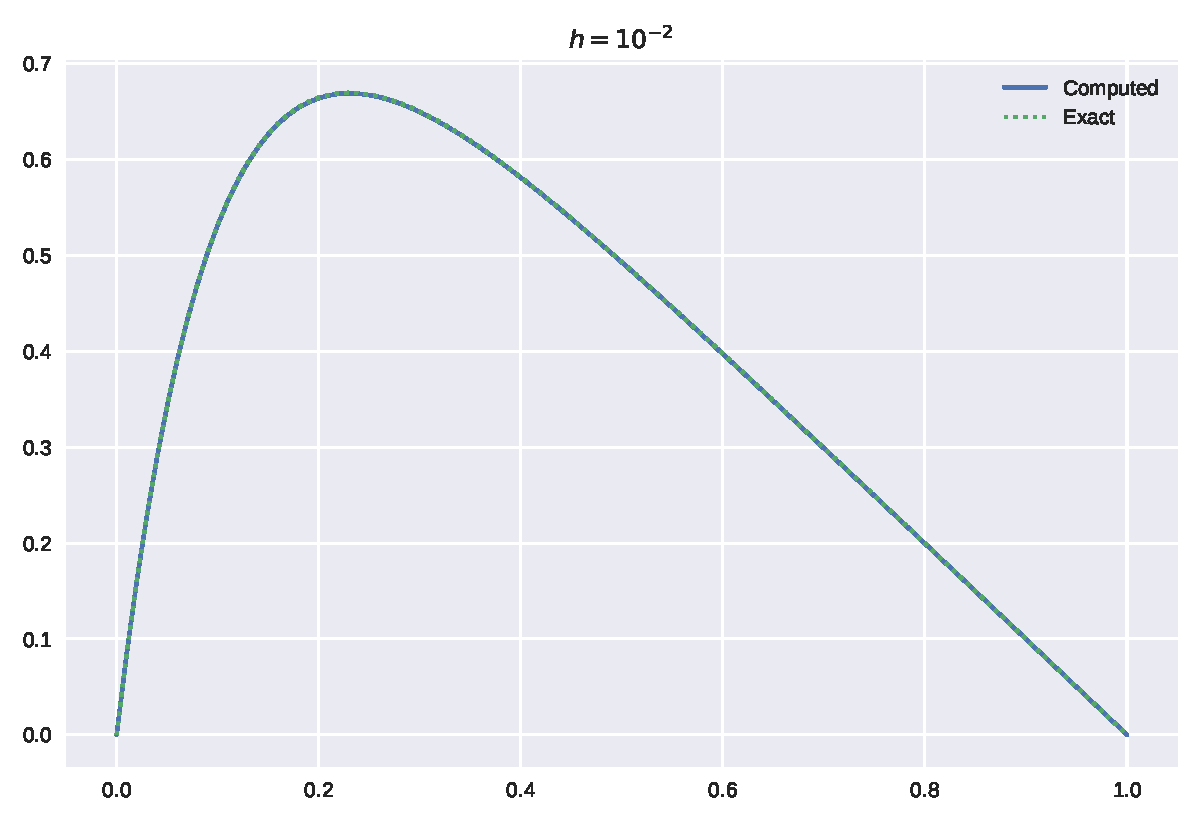
\includegraphics[scale=0.44]{../output/slow_2.pdf}
	\label{fig:slow_2}
	\caption{This figure shows the numeric solution for our general algorithm and the exact solution on top (green dashed line). The step size used is $h=10^{-2}$.} 
\end{figure}

\begin{figure}[h]
	\centering
	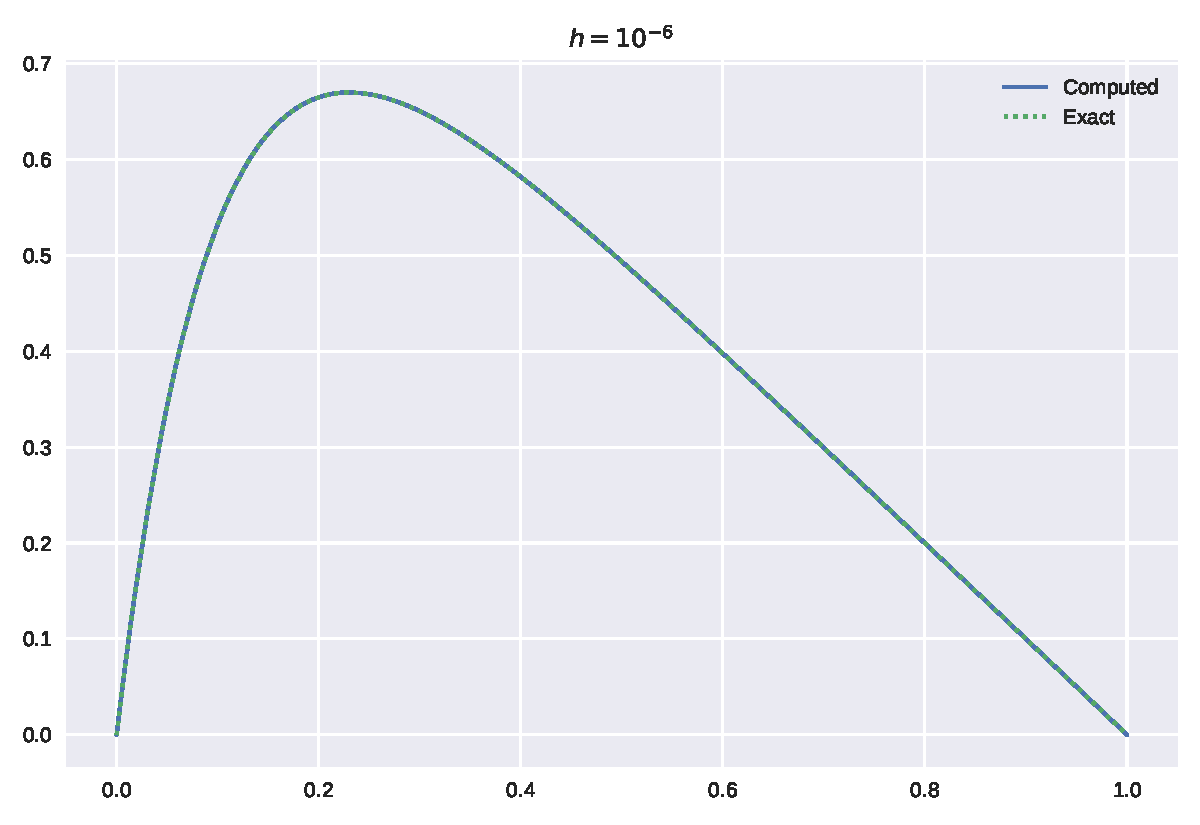
\includegraphics[scale=0.44]{../output/slow_6.pdf}
	\label{fig:slow_6}
	\caption{This figure shows the numeric solution for our general algorithm and the exact solution on top (green dashed line). The step size used is $h=10^{-6}$.} 
\end{figure}

\begin{table} [h]  %[p] % Uncomment to put table in Appendix
	\begin{tabular}{||c | c||}
			\hline
			$\log_{10}(h)$ & $\epsilon$    \\ \hline
			-6 & -6.08    \\ \hline
			-5 & -8.84    \\ \hline
			-4 & -7.08    \\ \hline
			-3 & -5.08    \\ \hline
			-2 & -3.08    \\ \hline
	\end{tabular}
	\caption{This table shows the relative error for our general method. The firs column is the logarithm of our step size and the second column is the relative error (see figure \ref{fig:slow_error} for table plotted).}
	\label{tab:slow_error}
\end{table}


\begin{figure}[h]
	\centering
	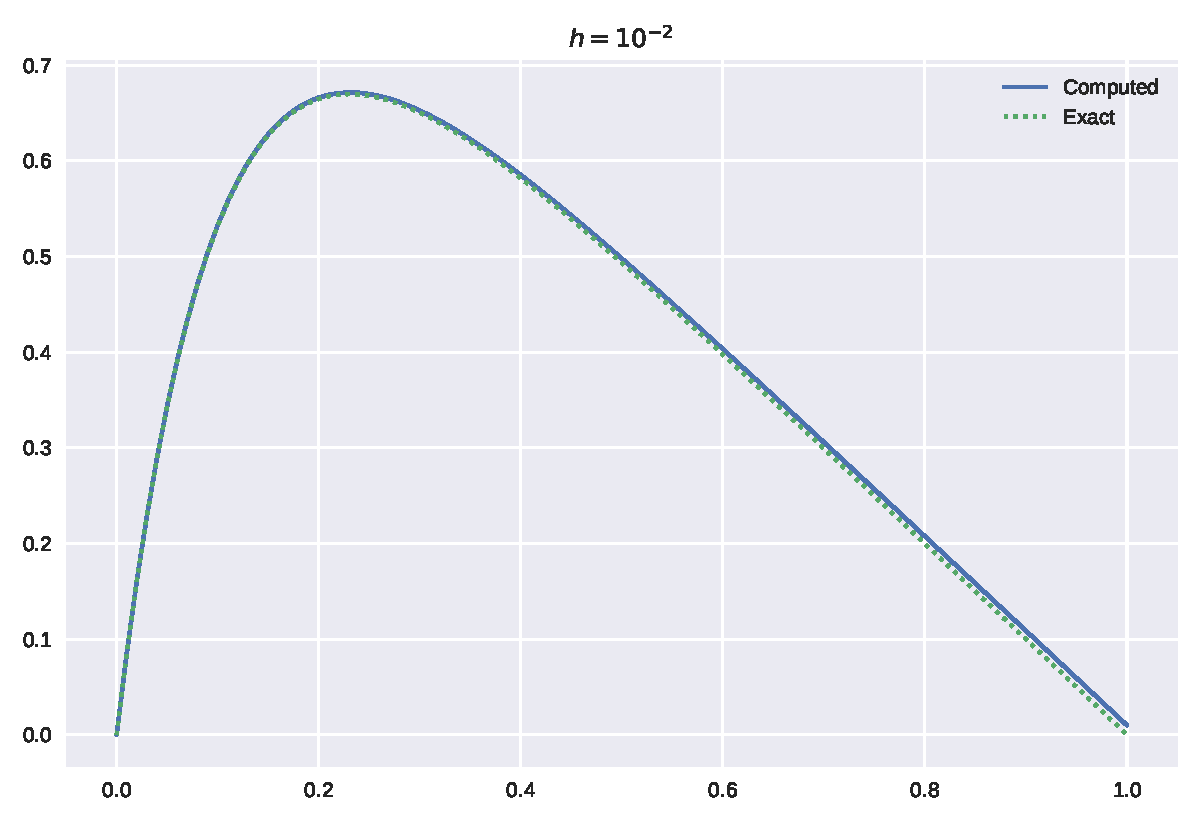
\includegraphics[scale=0.5]{../output/fast_2.pdf}
	\label{fig:fast_2}
	\caption{This figure shows the numeric solution for our specific algorithm and the exact solution on top (green dashed line). The step size used is $h=10^{-2}$.} 
\end{figure}

\begin{figure}[h]
	\centering
	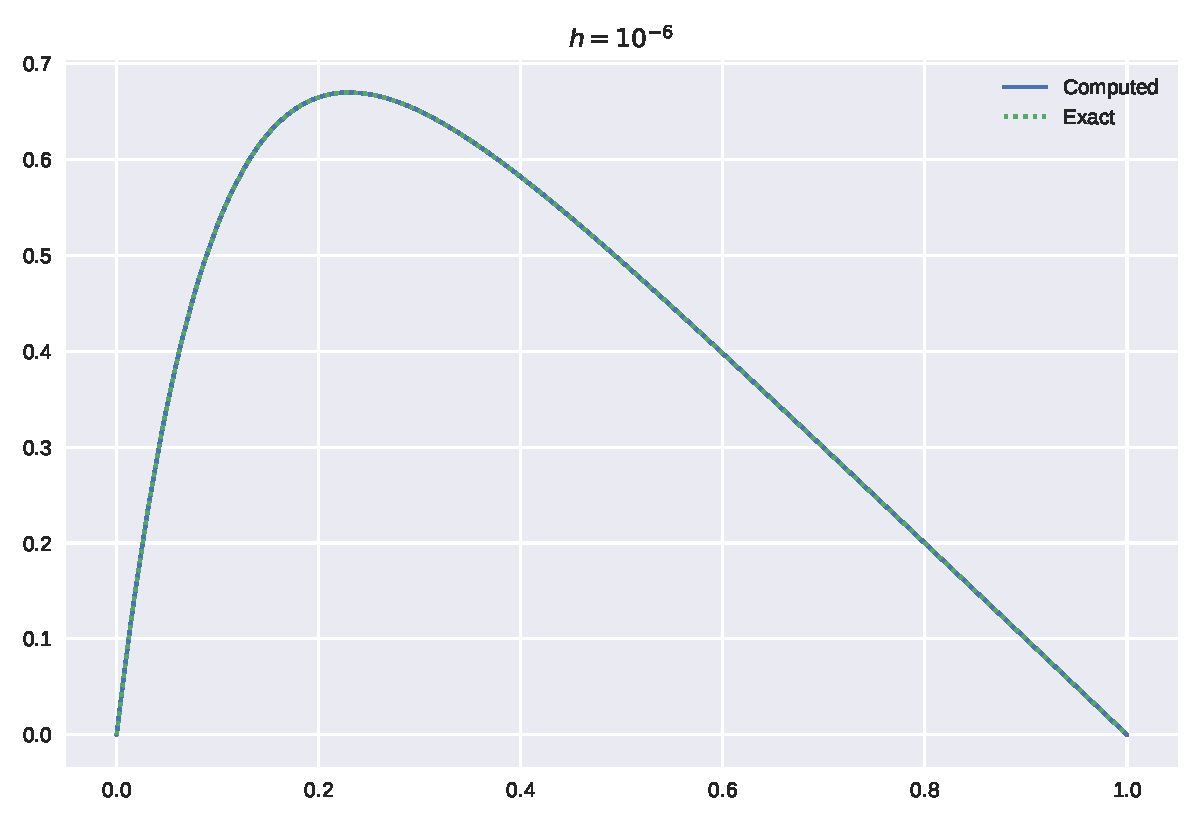
\includegraphics[scale=0.5]{../output/fast_6.pdf}
	\label{fig:fast_6}
	\caption{This figure shows the numeric solution for our specific algorithm and the exact solution on top (green dashed line). The step size used is $h=10^{-6}$.} 
\end{figure}

\begin{table} [h]  %[p] % Uncomment to put table in Appendix
	\begin{tabular}{||c | c||}
			\hline
			$\log_{10}(h)$ & $\epsilon$    \\ \hline
			-7 & -9.65    \\ \hline
			-6 & -10.18    \\ \hline
			-5 & -9.08    \\ \hline
			-4 & -7.08    \\ \hline
			-3 & -5.08    \\ \hline
			-2 & -3.08    \\ \hline
	\end{tabular}
	\caption{This table shows the relative error for our specialized method. The firs column is the logarithm of our step size and the second column is the relative error (see figure \ref{fig:fast_error} for table plotted).}
	\label{tab:fast_error}
\end{table}


\begin{figure}[h]
	\centering
	\includegraphics[scale=0.5]{../output/lu_2.pdf}
	\label{fig:lu_2}
	\caption{This figure shows the numeric solution for the LU-algorithm and the exact solution on top (green dashed line). The step size used is $h=10^{-2}$.} 
\end{figure}

\begin{figure}[h]
	\centering
	\includegraphics[scale=0.5]{../output/lu_4.pdf}
	\label{fig:lu_4}
	\caption{This figure shows the numeric solution for the LU-algorithm and the exact solution on top (green dashed line). The step size used is $h=10^{-4}$.} 
\end{figure}
\section{Discussion}

\begin{table} [h]  %[p] % Uncomment to put table in Appendix
	\begin{tabular}{||c | c||}
			\hline
			$\log_{10}(h)$ & $\epsilon$    \\ \hline
			-4 & -7.08    \\ \hline
			-3 & -5.08    \\ \hline
			-2 & -3.08    \\ \hline
			-1 & -1.10    \\ \hline
	\end{tabular}
	\caption{This table shows the relative error for our LU decomposition method. The firs column is the logarithm of our step size and the second column is the relative error (see figure \ref{fig:lu_error} for table plotted).}
	\label{tab:lu_error}
\end{table}


\begin{figure}[h]
	\centering
	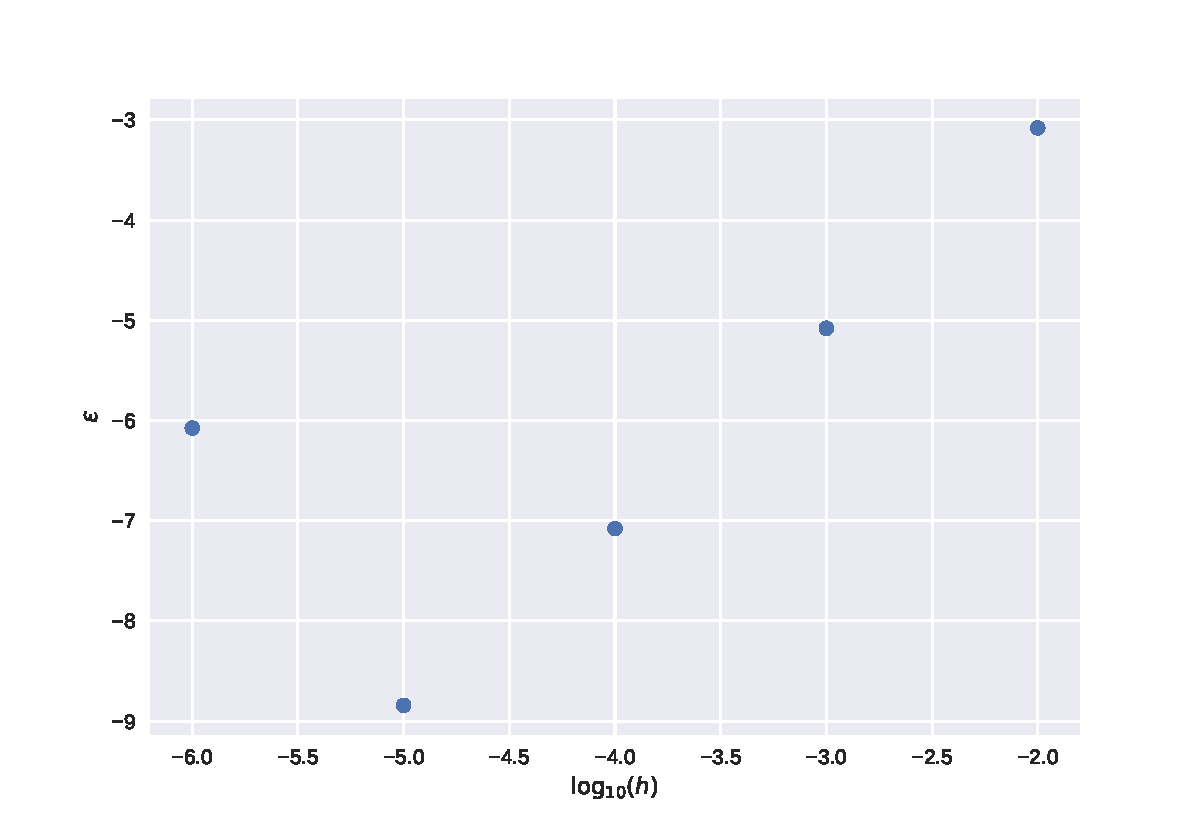
\includegraphics[scale=0.5]{../output/slow_errors.pdf}
	\label{fig:slow_error}
	\caption{Here we have the table of errors (table \ref{tab:slow_error}) from our general method plotted. Along the x-axis we have the logarithm of the step size ($log_{10}(h)$) and along the y-axis we have the relative error ($\epsilon$).} 
\end{figure}

\begin{figure}[h]
	\centering
	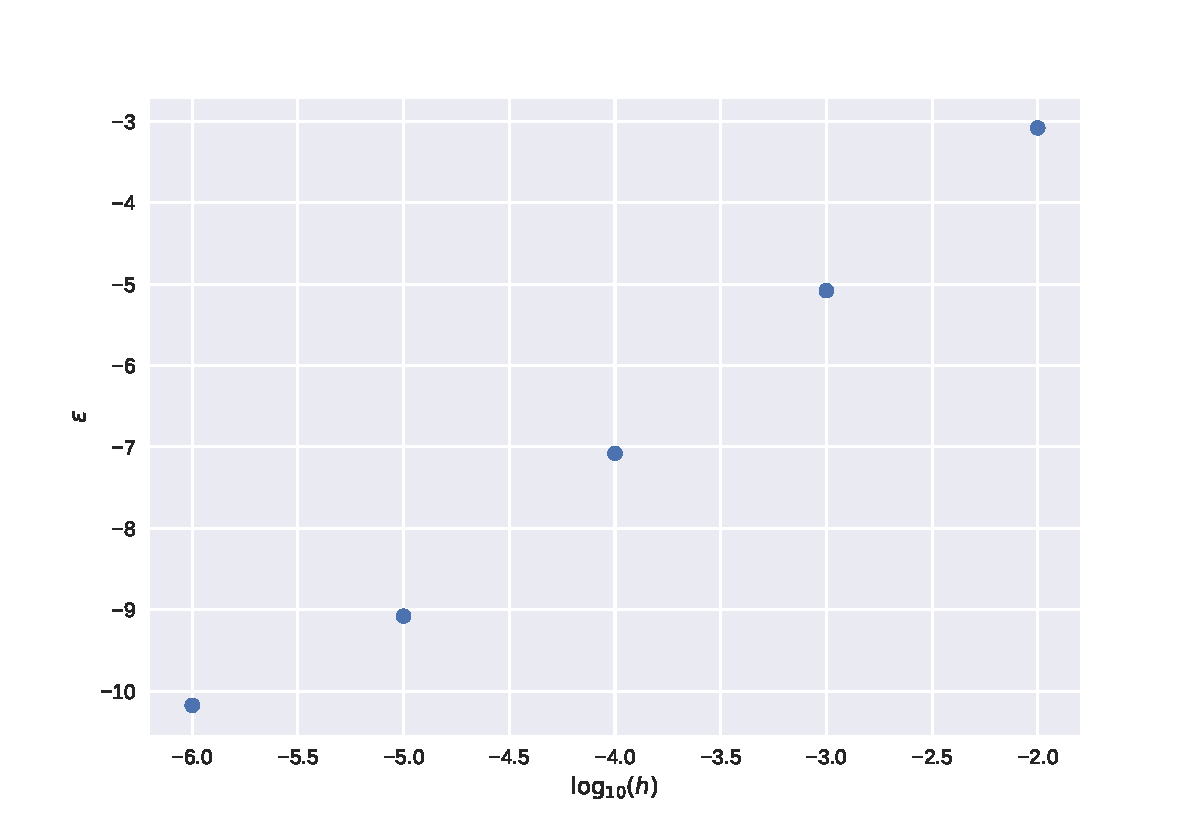
\includegraphics[scale=0.5]{../output/fast_errors.pdf}
	\label{fig:fast_error}
	\caption{Here we have the table of errors (table \ref{tab:fast_error}) from our specialized method plotted. Along the x-axis we have the logarithm of the step size ($log_{10}(h)$) and along the y-axis we have the relative error ($\epsilon$).} 
\end{figure}

\begin{figure}[h]
	\centering
	\includegraphics[scale=0.5]{../output/lu_errors.pdf}
	\label{fig:lu_error}
	\caption{Here we have the table of errors (table \ref{tab:lu_error}) from the LU decomposition method plotted. Along the x-axis we have the logarithm of the step size ($log_{10}(h)$) and along the y-axis we have the relative error ($\epsilon$).} 
\end{figure}

\begin{table}  %[p] % Uncomment to put table in Appendix
		\begin{tabular}{||c | c | c | c||}
			\hline
			$n$ & Slow [$\mu$s] & Fast [$\mu$s] & LU [$\mu$s]    \\ \hline
			$10^{1}$ & - & - & 140.00    \\ \hline
			$10^{2}$ & 2.60 & 2.00 & 2608.80    \\ \hline
			$10^{3}$ & 30.40 & 17.80 & 86337.00    \\ \hline
			$10^{4}$ & 572.60 & 200.60 & 10058519.80    \\ \hline
			$10^{5}$ & 7607.60 & 2741.00 & -    \\ \hline
			$10^{6}$ & 35499.80 & 14172.00 & -    \\ \hline
		\end{tabular}
	\caption{This table shows the time used for the different algorithms in microseconds. The first column is the number of steps used, second the general algorithm, third the specialized one and the third correspond to the LU decomposition.}
	\label{tab:time}
\end{table}

\section{Conclution}

\onecolumngrid
\vspace{1cm} % some extra space
\newpage
\begin{thebibliography}{}
\bibitem {oppgavetekst} HER REFERERERERERER VI TIL OPPGAVETEKSTEN
\bibitem {lu} HER REFERERERERERR VI TIL LU (https://mathworld.wolfram.com/LUDecomposition.html)
\bibitem {lu_wiki} https://en.wikipedia.org/wiki/LU\_decomposition
\bibitem {github} https://github.com/sigurdru/FYS3150/tree/sigurd/Project1
\bibitem {armadillo} http://arma.sourceforge.net/
\end{thebibliography}

\section{Appendix}


\section{Kode}

% \subsection{\textit{main.py}}
% \lstinputlisting[language=Python]{../main.py}
%
% \subsection{Output fra \textit{main.py}}
% \verbatiminput{../main_output.txt}



\end{document}
